\documentclass[10pt]{beamer}

\usetheme[progressbar=frametitle]{metropolis}
\usepackage{appendixnumberbeamer}

\usepackage{booktabs}
\usepackage[scale=2]{ccicons}

\usepackage{pgfplots}
\usepgfplotslibrary{dateplot}

\usepackage{hyperref}

\usepackage{xspace}
\newcommand{\themename}{\textbf{\textsc{metropolis}}\xspace}

\title{Football Datasets}
%\subtitle{}
% \date{\today}
\date{}
\author{Jonas Stillhard}
\institute{Swiss Federal Research Institute WSL\\
\href{mailto:jonas.stillhard@wsl.ch}{jonas.stillhard@wsl.ch}}
\titlegraphic{\hfill
\includegraphics[height=1.5cm]{logo.png}}

\begin{document}

\maketitle

%\begin{frame}{Table of contents}
%  \setbeamertemplate{section in toc}[sections numbered]
%  \tableofcontents[hideallsubsections]
%\end{frame}

%\section{Introduction}

\begin{frame}[fragile]{Motivation}
   \begin{itemize}
        \item Worldcup 2018 in Russia
        \item Focus on Football
        \item Potential for a widely received publication / blog post 
      \end{itemize}
\end{frame}


\begin{frame}[fragile]{Available Datasets}

\begin{itemize}
\item \href{https://github.com/openfootball}{\textbf{Openfootball aka football.db:}} Available on github. Can be downloaded to a sqLite database via command prompt using ruby. Very convenient. Provides scores for all fixtures since 1930. 
\item \href{http://www.football-data.co.uk/data.php}{\textbf{footballdata.uk:}} Provides final scores for 10 european countries and 22 leagues including betting odds. Updated weekly, data is available as .csv, data goes back to 1994. Very interesting dataset, might be useful for other analyses. 
\item \href{https://github.com/jalapic/engsoccerdata}{\textbf{engsoccerdata:}} Historical football datasets with a focus on english premier league, historical data back to 1871. Available on github.
\item Check out
\href{https://www.jokecamp.com/blog/guide-to-football-and-soccer-data-and-apis/#openfootball}{\textbf{Joe Kampschmidts}} blog for more datasets and API's. 
\end{itemize}
\end{frame}

%\begin{frame}[fragile]{The openfootball / football.db dataset}
%The database contains 35 tables of which only very few might be of interest. \\
%A dataset containing the following columns has been created (we might also discuss on an optimal structure for that data)

%\end{frame}

\begin{frame}[fragile]{Restrictions}

\begin{itemize}
\item Predictions of final scores and winners of tournaments integrating as much predictors/variables as possible are very common - e.g.,  Bloomberg tried to predict the winner in 2014. 
\item Data availability is not restricted if using more general data (e.g., final scores). 'Fancier' data (e.g., position of players when scoring goals) are not available. 
\end{itemize}
\end{frame}


{\setbeamercolor{palette primary}{fg=black, bg=yellow}
\begin{frame}[standout]
  Ideas?
\end{frame}
}

\begin{frame}[fragile]{Preliminary ideas}

\begin{itemize}
\item Use available datasets. 
\item The goal is \textbf{not} to outperform existing models
\item Provide rules of thumb for teams that win and make these rules as easy as possible (e.g., countries starting with A, B, C, D, E, F will always win if playing against another country).
\item Benchmarking: Use real world data if available (we might get a world cup 2014 office pool dataset from Switzerland (N>1000)) or betting odds.
\end{itemize}

\end{frame}

\begin{frame}[fragile]{'No clue, here's what you do'}

\begin{itemize}
\item  Provide people not interested in football with good rules of thumb so they can perform all right in an office pool. 
\item What strategies are most promising for different types of betting pools?
\item Depending on the amount of time one is willing to invest for an (office) pool, what is the best strategy (e.g., if you are willing to have a look at the betting odds every day, follow these, else always bet on a 1:0).
\item The main goal is not to win money but to maximize social standing with a minimum effort. 
\end{itemize}

\end{frame}

\begin{frame}[fragile]{Preliminary analyses}
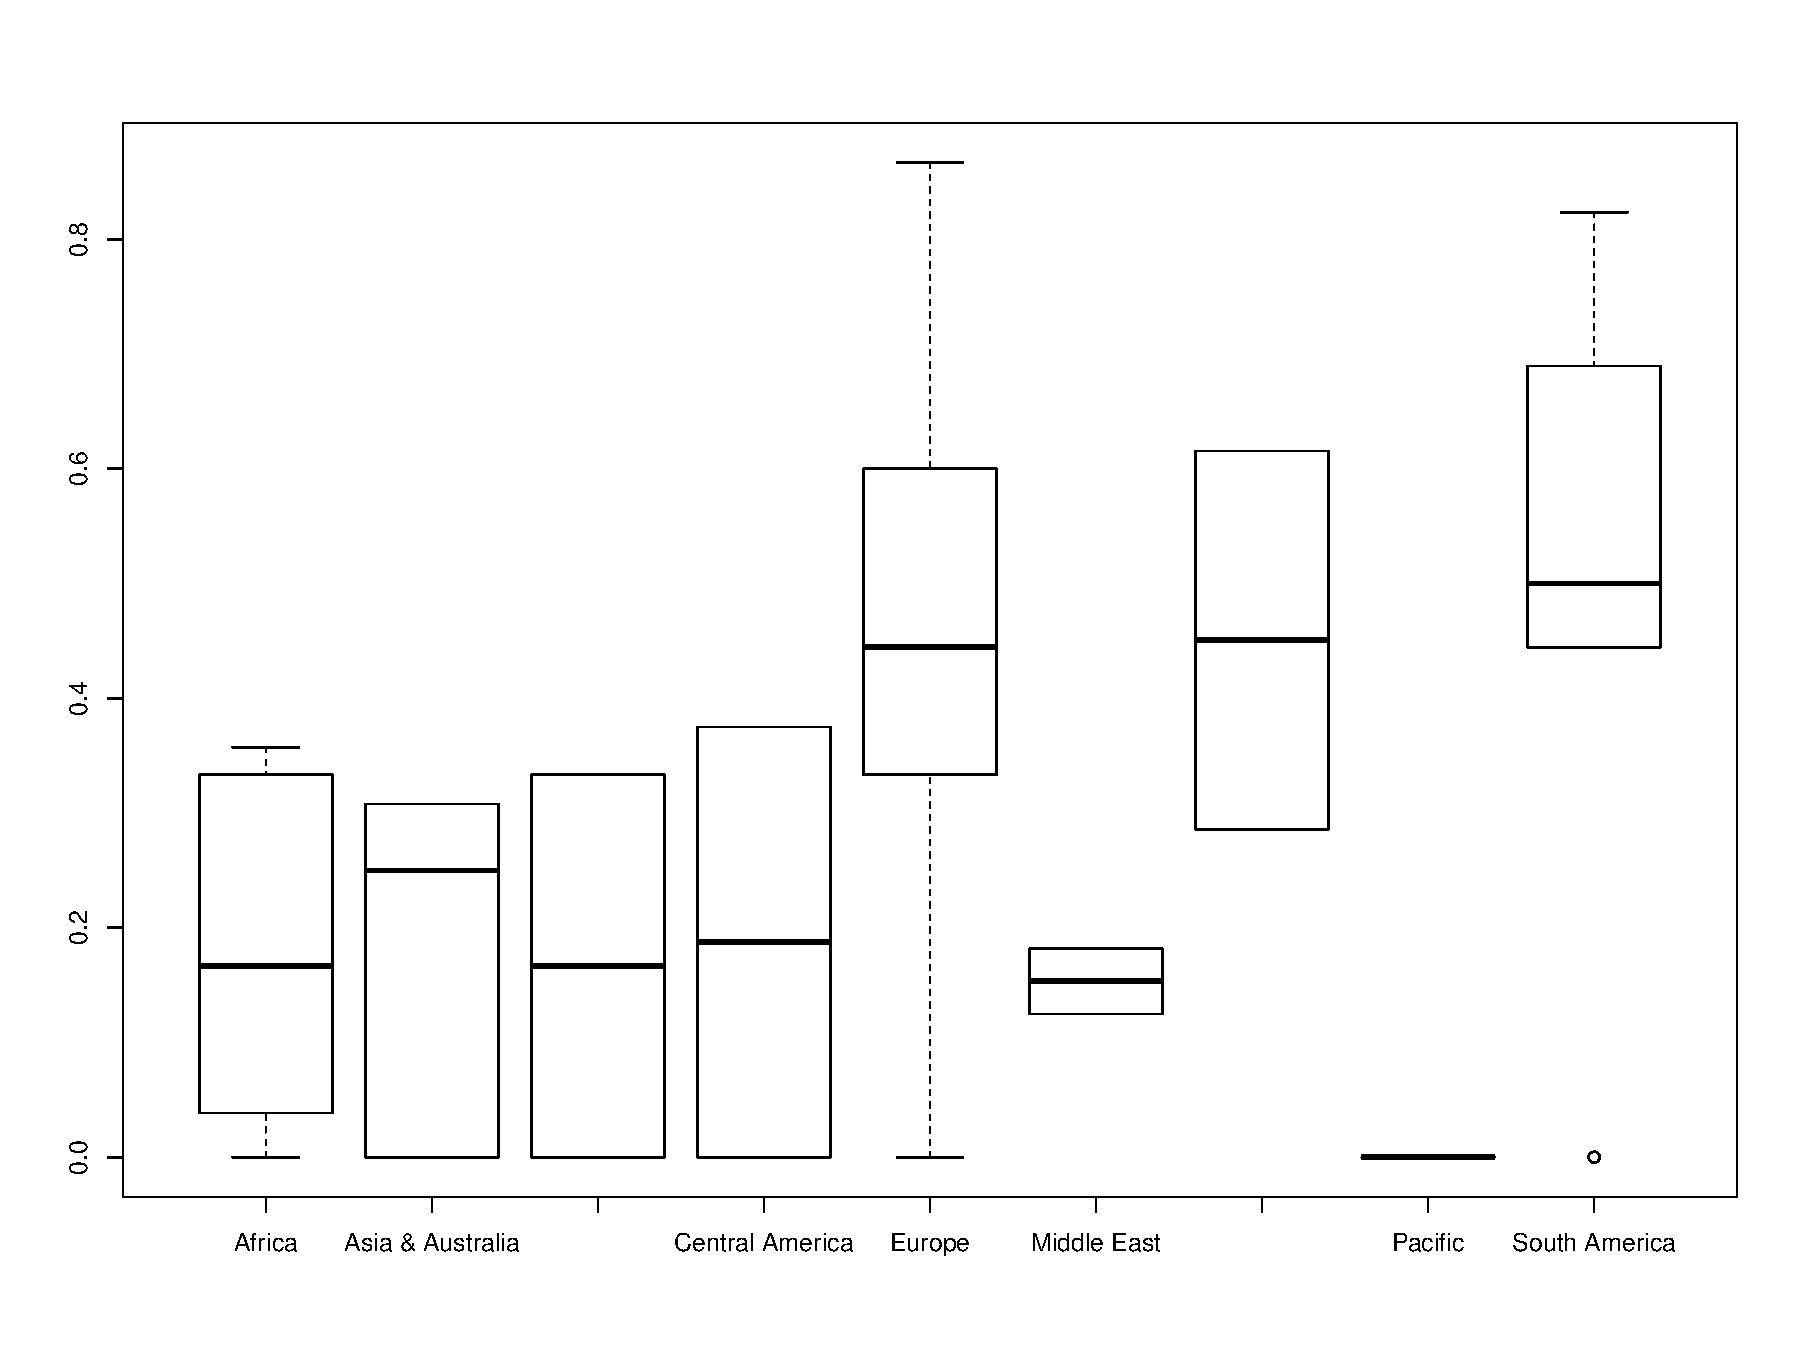
\includegraphics[scale=0.15]{winpercentage.pdf}
\end{frame}

\begin{frame}[fragile]{Data}

The data is available on github in a private project, do not hesitate to request access.
So far, the dataset contains all world-cup games until 2010. Due to a bug, the data of the 2014 world cup can not be downloaded at the moment.  

\url{https://github.com/jstillh/ftblData.git}
\end{frame}

{\setbeamercolor{palette primary}{fg=black, bg=yellow}
\begin{frame}[standout]
  Questions?
\end{frame}
}


%\begin{frame}[allowframebreaks]{References}
%
%  \bibliography{demo}
%  \bibliographystyle{abbrv}

%\end{frame}

\end{document}
